%\documentclass[12pt,oneside,a4paper,english]{article}
\documentclass{article}
%\usepackage[margin=2.5cm]{geometry}
\usepackage{amsmath}
\usepackage{booktabs}
\usepackage[T1]{fontenc}
\usepackage[utf8]{inputenc}
%\usepackage[latin2]{inputenc}
%\usepackage[margin=2.25cm,headheight=26pt,includeheadfoot]{geometry}
\usepackage[english]{babel}
\usepackage{listings}
\usepackage{color}
\usepackage{titlesec}
\usepackage{titling}
\usepackage[framed, numbered]{matlab-prettifier}
\usepackage{changepage}
\usepackage{amsmath}
\usepackage{hyperref}
\usepackage{enumitem}
\usepackage{graphicx}
\usepackage{subcaption} 
\usepackage{fancyhdr}
\usepackage{lastpage}
\usepackage{caption}
\usepackage{tocloft}
\usepackage{setspace}
\usepackage{multirow}
\usepackage{titling}
\usepackage{float}
\usepackage{comment}
\usepackage{booktabs}
\usepackage{indentfirst}
\usepackage{lscape}
\usepackage{booktabs,caption}
\usepackage[flushleft]{threeparttable}
\usepackage[english]{nomencl}
\usepackage{xcolor}
\usepackage{lipsum}
\usepackage{url}
\usepackage[backend=biber,style=ieee]{biblatex}


% --- set footer and header ---
\pagestyle{fancy}
\fancyhf{}

\setlength{\parindent}{2em}
\title{Case 2} % to reference as \title, dont use \maketitle
\author{02582 Computational Data Analysis \\ \\ Group 14 - s224766, s224381, s224360 \& s215141}
\date{\today}
%\makeatletter\let\Title\@title\makeatother

\lstset{language=Matlab,
style=Matlab-editor,
basicstyle=\normalsize\mlttfamily,
numbers=left,
numberstyle={\scriptsize\color{black}},			% size of the numbers
numbersep=0.5cm											
}

\newlist{steps}{enumerate}{1}
\setlist[steps, 1]{leftmargin=1.5cm,label = Step \arabic*:}
\renewcommand{\headrulewidth}{1pt}
\renewcommand{\footrulewidth}{1pt}

%\lhead{\Title}
\rhead{\nouppercase{\rightmark}}
\lhead{Case 2 group 14}
\rfoot{\includegraphics[height=1.25cm]{root/logo.pdf}} % right header logo
\setlength\headheight{16pt}
\setlength{\footskip}{50pt}
\lhead{Case 2 group 14} %rightH title
\usepackage{lastpage}
\fancyfoot{}
\cfoot{\thepage/\pageref{LastPage}}
\pagenumbering{arabic}



% --- End of page settings ---

\addbibresource{document.bib}

\begin{document}
\pagenumbering{roman} 
%\input{sources/0_frontpage.tex}
\maketitle

\doublespacing
%\addcontentsline{toc}{section}{Table of Contents}
\renewcommand{\baselinestretch}{1}\normalsize

\renewcommand{\baselinestretch}{1}\normalsize
%\singlespacing
\thispagestyle{fancy} % force page style

\pagenumbering{arabic} 
\fancyfoot[C]{Page \thepage\ of \pageref{LastPage}}

\title{Case 2}


\section*{Introduction and Data description}

\noindent
This task consisted of an exploratory and unsupervised analysis of the dataset EmoPairCompete~\cite{datasource}. EmoPairCompete is based on biosensory data from participants of an emotional study, measuring the stress levels of different participants during a puzzle exercise. Additionally to the biosignal data (including heart rate, blood volume pulse (BVP), electrodermal activity (EDA) and temperature) the participans also answered a range of questions after each phase of the experiment, to measure their levels of stress. Exactly these responses and biosensor measures are what we aim to gain an understanding of, how does the body and mind react in situations of high pressure and competition?  This concludes in the question, determine if a person is in a stressful situation through quantification of their mind and body?

\textcolor{yellow}{We need to update the aim when frederiks stuff is done :DD}

\textcolor{red}{I think we in the introduction need to answer the following questions: Formulate a clear purpose for your project, so the aim of your analysis is clear. What are your research questions? What kind of representation would you like to derive from the features of the biosignals? What could it be used for? We expect you to use methods from the course curriculum. }


\subsection*{Data overview}
\noindent
The provided dataset inlcudes the raw data as well as two preprocessed dataframes, one \texttt{HR$\_$data.csv} and the updated \texttt{HR$\_$data2.csv}. 
\noindent
The raw data consists of data from 6 different days and 26 different people, where each person went though 4 rounds of experiments, where each rounds is split in three phases. The three phases where a pre-puzzle phase, a during puzzle phase and a post puzzle phase, where during each the biosensor measured heart rate, BVP, EDA and temperature. After each phase a questionnaire was answered, reporting the feelings of each person, including frustrated, upset, hostile, alert, ashamed, inspired, nervous, determined, attentive, afraid, active and lastly how difficult they found the task. 
\\
\noindent
Each day has a \texttt{team$\_$info.csv} file, indicating the teams of 2, and who is the puzzler in each team. 
\\
\noindent
To maintain full control over the data pipeline, we opted to work directly with the raw data rather than the preprocessed versions provided through the course material.

\begin{figure}[H]
    \centering
    
\includegraphics[width=0.8\linewidth]{figures/person1_plot.png} %FIX ME: plot title is wrong, says "round 1 & phase 1", when it should just say "round 1"
    \caption{On the plot is shown the raw data of the four different parameters measured by the biosensor. In this case it is the first person (day 1, person 1) through the first round and all three phases.}
    \label{fig:person_1_raw}
\end{figure}

\subsection*{Preprocessing}
\subsubsection*{Collecting personal data}
\noindent
To utilize the raw time series data we have collected all the biosensor data in one dataframe per person labelled \texttt{Person\{i\}\_\{DayID\}\_\{PersonID\}.csv} where $i \in \{1,...,26\}$  is the number of participans with usable data.
This means that all rounds and phases of each person where combined, with the column \textit{time} being the primary key, as one person can only be one place at a time.
\\
\noindent
The questionary responses we also collected for each round and phase in data-frames named \texttt{Person\{i\}\_\{DayID\}\_\{PersonID\}\_responses.csv}
\textcolor{red}{Lastly, to ensure systematic oversight of the data, a dictionary of information of each person was created. This dictionary included start and end timestamps of all rounds and phases, as well as group ID and if they were a puzzler or not. WE DONT END UP USING THIS, REMOVE?}

\subsubsection*{Normalization and extraction of features}
After preprocessing the raw biosignal data into individual frameworks, we normalize the data for each person using exclusively their 'Phase1' baseline period. Then, using a sliding window each persons data is aggregated into 30 second intervals, in a manner that prevents a given window to overlap from one phase or round into the next (in case of any remaining <30 seconds in the phase after the aggregation we would consider this as one smaller window). For each 30 second segment we extract the mean, standard deviation, min and max values for the four biosignals, and additionally the peak counts for EDA and slope for TEMP. By discarding the "HR\_data" files, working directly with the raw temporal domain data, applying the 30 seconds rolling windows and extracting our own features we are satisfying the advanced challenge: Temporal Dynamics \& Feature Engineering. Normalizing by the baseline for each person before extracting features rather than the other way around means we  also account for the per-participant differences such as resting body temperature or resting heart rate.

\section*{Model and method}
\subsection*{One-class support vector machine}
\noindent
We choose to analysis the bio signal and response data from a \textbf{Zero-Shot Stress Detection} point of view, where we employ an unsupervised One-Class Support Vector Machine (OC-SVM) Model. We train the model solely on the ’Resting’ phase with the objective of being able to label any other phase ('puzzling' and 'post-puzzling ') as anomalies.

We pick a SVM model as we expect to see a great deal of overlap in the bio-signals across phases. We therefore opt for a model that is adaptable to this challenge, i.e. SVMs.
Secondly the use of SVM allows us to use the Kernel trick.  The Kernel Trick allows a model to operate in a high-dimensional feature space without ever explicitly calculating the coordinates of the data in that space. Instead of performing a basis expansion h(X), we define a Kernel function $\mathcal{K}(x_i,x_j)$ that represents the inner product of those expanded features: $\mathcal{K}(x_i,x_j)=\langle h(x_i),h(x_j)\rangle$. 
In other worrds the kernel trick allows us to calculate geometric relationships in infinite dimensions without actually
mapping the data there.\\ \textcolor{red}{source here?}

We make use of the RBF kernel given by:  
$\mathcal{K}(x,x')=e^{-\gamma||x-x'||^2}$
which mathematically represents a dot product in an infinite-dimensional space.  We choose this kernel as it allows us "form a none linear relationships"  and the biosignals are none linear \textcolor{red}{(we think??) source}

One-Class SVM deviates from standard SVP by instead of separating N classes from each other, One-Class SVM defines a single 'normal class' from data and is then able to single out anomaly inputs that does not fit within this class. This makes it an ideal model for stress detection. 


There are some downsides related to this model choice: \textcolor{red}{what is the purpose of the points below? should they stay?} 
\begin{itemize}
    \item Kernel methods do not scale well. Limited to around 10,000-20,000 observations
    \item Kernel methods generally do not do variable selection in any reasonable or automatic way
    \item With more features than observations there is always a separating hyperplane
    \item Actually infinitely many which we have to choose between
    \item Potential problem with large number of features if many of them are garbage
    \item SVM does not generalize gracefully when the number of classes are more than two
    \item Frequently used for multiclass classification anyway
\end{itemize}

\subsection{Gaussian mixture model}
\textcolor{red}{something here}

\subsection*{Model selection}
% \textcolor{red}{this section needs to take both models into account, and maybe be a but more fluent}

% We use K-fold-Cross validation
% \textcolor{red}{Model Assessment (Outer Split): Separate 5 subjects $( \approx 20\%)$ as a "vaulted" test set. They are never seen by the model during the tuning of hyperparameters.  }

% Model Selection (Inner Loop): Use the 21 remaining subjects for 5-fold cross-validation.  
% Train: 80\% of these 21 subjects (~17 people) are used to fit the model weights $\alpha$i.  

% Validate: $20\%$ ($\approx$ 4 people) are used to calculate the True Negative Rate (identifying 'Resting' as normal) to choose optimal $\gamma$ and $\nu$.  
% Final Prediction: Apply the selected best model to the 5 vaulted subjects to report the final Zero-Shot Stress Detection rate.

% The final model is configured and selected in the following way: 
% first we do all the preprocessing and normalization and sliding window. 
% 2) We train the model using cross validation soley on the 'resting' data (training on 80 percent and then seeing how many of the points from the remaining thirty percent are outaside the defined boundary. From this method we update and congregation the gamma and c values 

%  C definiens the kernel boundary, High values lead to a "wiggly" boundary (high variance); low values lead to a smooth boundary (high bias). Support Vectors: The ’difficult’ points on the margin edges. They dictate the boundary.
% • Safe Points: The ’easy’ cases. Once the model is trained, these points carry zero information. SO C helps decide which points to become support vectors, 

% We also adjust the Gamme? Lambda? loss regularization? defining the amount of points from the restings phases we use for testing that we will allow to be labed as outliers, and thus not include within out decision boundary. 

% We then ones we have determined out hyper parameters asses the performance testing it on an unseen persons (determine amount) stress and resting phases and see how often it quesses correctly. 
To perform strictly the "zero-shot" anomaly detection we employ a Leave-One-Subject-Out (LOSO) Cross-Validation scheme. This is where we iterate through each of the 26 subjects, isolating them one-by-one, training the GMM and SVM model only on the Resting, "Phase1" of the remaining 25 subjects and then use this trained model to detect how anomalous each phase of the isolated subject is. Crucially, the models are only trained and tuned on Phase 1 data. Prior to the modeling part we use `StandardScaler` to scale all the extracted features to zero their means and make their standard deviations one. We then perform dimensionality reduction using Principal Component Analysis retaining components that explain 95\% of variance. Both the scaling and dimensionality reduction are performed within the cross-validation loop preventing data leakage. For the OC-SVM model, $\nu$ and $\gamma$ parameters are tuned on the inner loop subjects, the parameters explored were $\nu \in [0.05, 0.10, 0.15, 0.20, 0.25]$ and $\gamma \in [\text{scale}, \text{auto}, 0.1, 0.01]$. Where the optimal combination is chosen by finding the lowest Calibration Error on the inner validation subjects (i.e. if it is $\nu = 0.10$, then the best model would classify exactly 10\% of data as anomalous). The GMM model was also tuned on inner loop subjects, here minimizing the Bayesian Information Criterion (BIC) for different numbers of distributions. To ensure a fair comparison, we applied the empirically tuned baseline allowed outliers $\nu$ from the SVM model to also be the percentile threshold for the GMM model.

\textcolor{red}{THINGS TO THINK ABOUT: }\\
\textcolor{red}{- is the nu and gamma the same for both models? look into course mateiral}\\
\textcolor{red}{The kernel used, is it okay to use in both of them }

\subsection*{Missing values}
\subsubsection*{Biosensor data}
Working with the raw datafiles meant dealing with missing values. We checked for missing values in all the biosensor data, that is the \texttt{BVP.csv}, \texttt{TEMP.csv}, \texttt{HR.csv} and \texttt{EDA.csv} files, but did not find any missing entries. Our assumption is that this is a product of the way the E4 biosensor collects and saves data. That is that if there is a 'missing value' in the recording, then the nature of for example how HR is measured, the recording will smooth over that. Other than the absence of missing values in the dataframes themselves, the time-intervals between each timestamp was also identical within all the datasets. 

\subsubsection*{Response data}
The response files had unlike the biosensor data instances of missing values. That is missing responses within some of the columns of the questionary that participants had to answer. There are missing values in 25 of the 312 files, one file with 4 missing entries, and 24 with only one missing entries. Most missing values (75\%) were in the category \textit{dificulty}, and was only missing in the pre and post puzzle ling phase except for once in the puzzling phase. This however is expected as the participants were only supposed to assess \textit{difficulty} in phase 2, and since we aim to separate the phase 1 from 2 and 3, this column becomes negligible.\\
\\
\noindent
Since we have opted to only use the biosensor data in as a training basis, the missing values in the response sheets do not create any issues for the model. We do however compare the responses with the corresponding average anomaly rating for each phase of each person. This is done as a way to evaluate and perspective our model to the personal responses of each person, and if missing values occur, then we simply do not compare those observations. We have chosen not to use imputation to fill in the gaps as the data is categorical, and though we could add an extra category of 'missing' it was decided that it would not add any value in our user case.


\subsection*{Factor handling}
As mentioned in the Missing values section, we are working with categorical response data, namely discrete values from either 0-5 or 0-10. All categorical classes had 'bad' ratings at 0, and 'good' at 5 or 10 according to the range. Though the information is categorical, it is clearly ordinal, and therefore we decided to normalize them using means and standard deviations (std) from each response class and person. We subtract mean to combat the bias of the general tendency of rating, that is if a person tends to rate generally high or low. A bias in the personal range of ratings can also skew the data, which is combated by the division with std.



\textcolor{red}{- Med categoriske data normaliseret som vi gør er vi mere prone til at få værdier på 0, hvis participans ikke ændrer deres var mellem phases, men i den phase skulle vi også gerne ikke se nogen høj anomality}


\textcolor{red}{The puzzler id (we dont use before the review with responses), responses are categorical but we currently normalize them by subtracting the mean}


\section*{Model validation}
This is how we performed our model validation and estimated the EPE

\section*{Results}
This is my chosen model (the best model).... Those are our results and our estimate of the EPE (given
as an estimate of RMSE).


\begin{figure}[H]
\begin{adjustwidth}{-1cm}{-1cm}
    \centering
    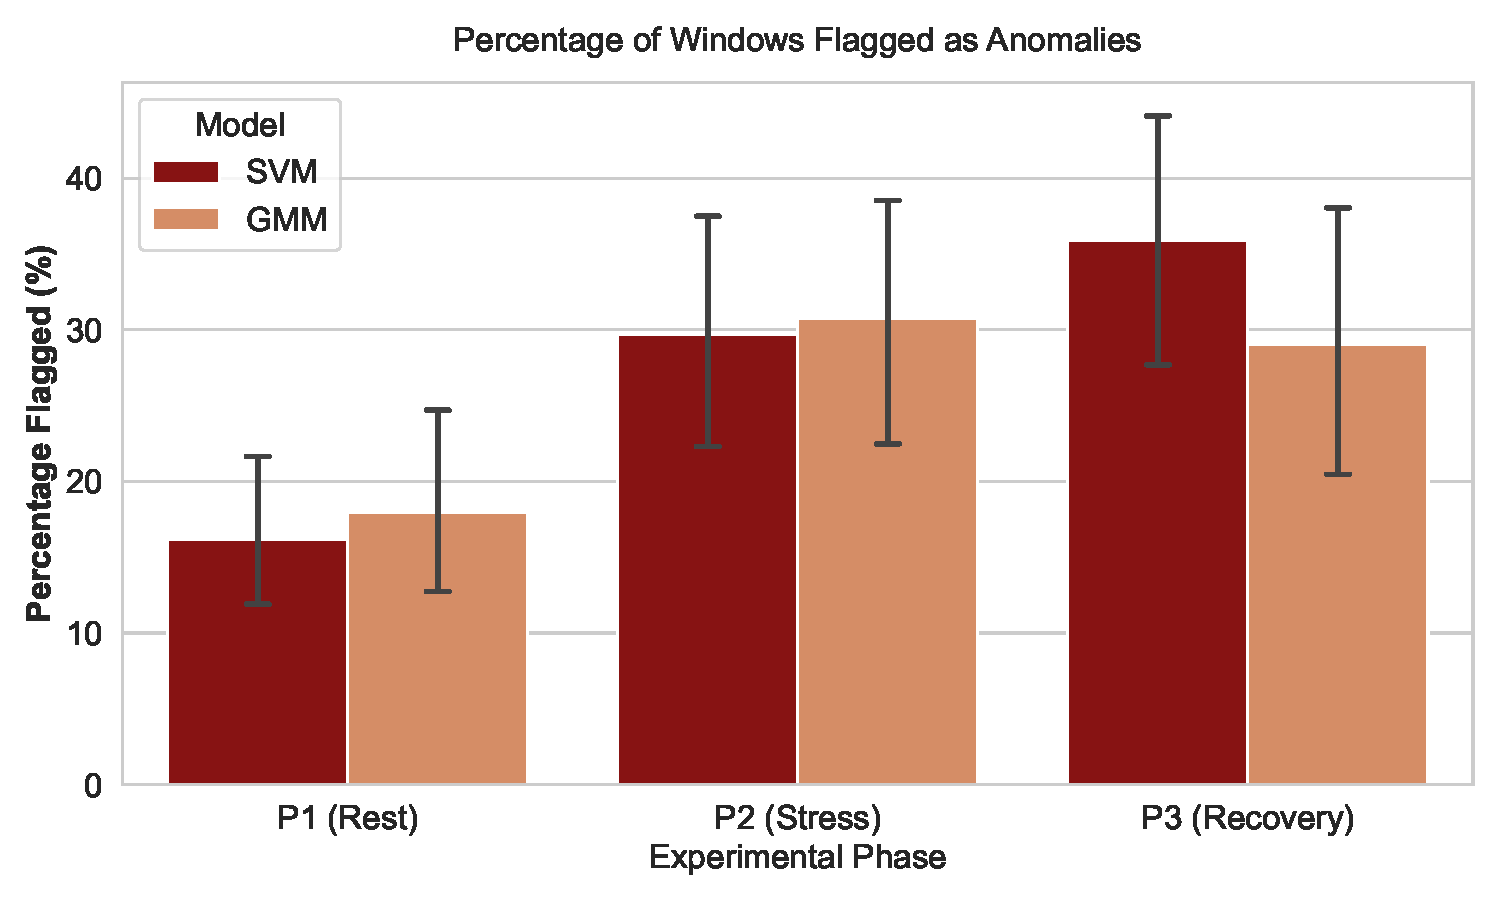
\includegraphics[width=0.8\linewidth]{figures/phase_anomalies.pdf}
    \caption{Caption}
    \label{fig:responses_correction}
\end{adjustwidth}
\end{figure}

\begin{figure}[H]
\begin{adjustwidth}{-2cm}{-2cm}
    \centering
    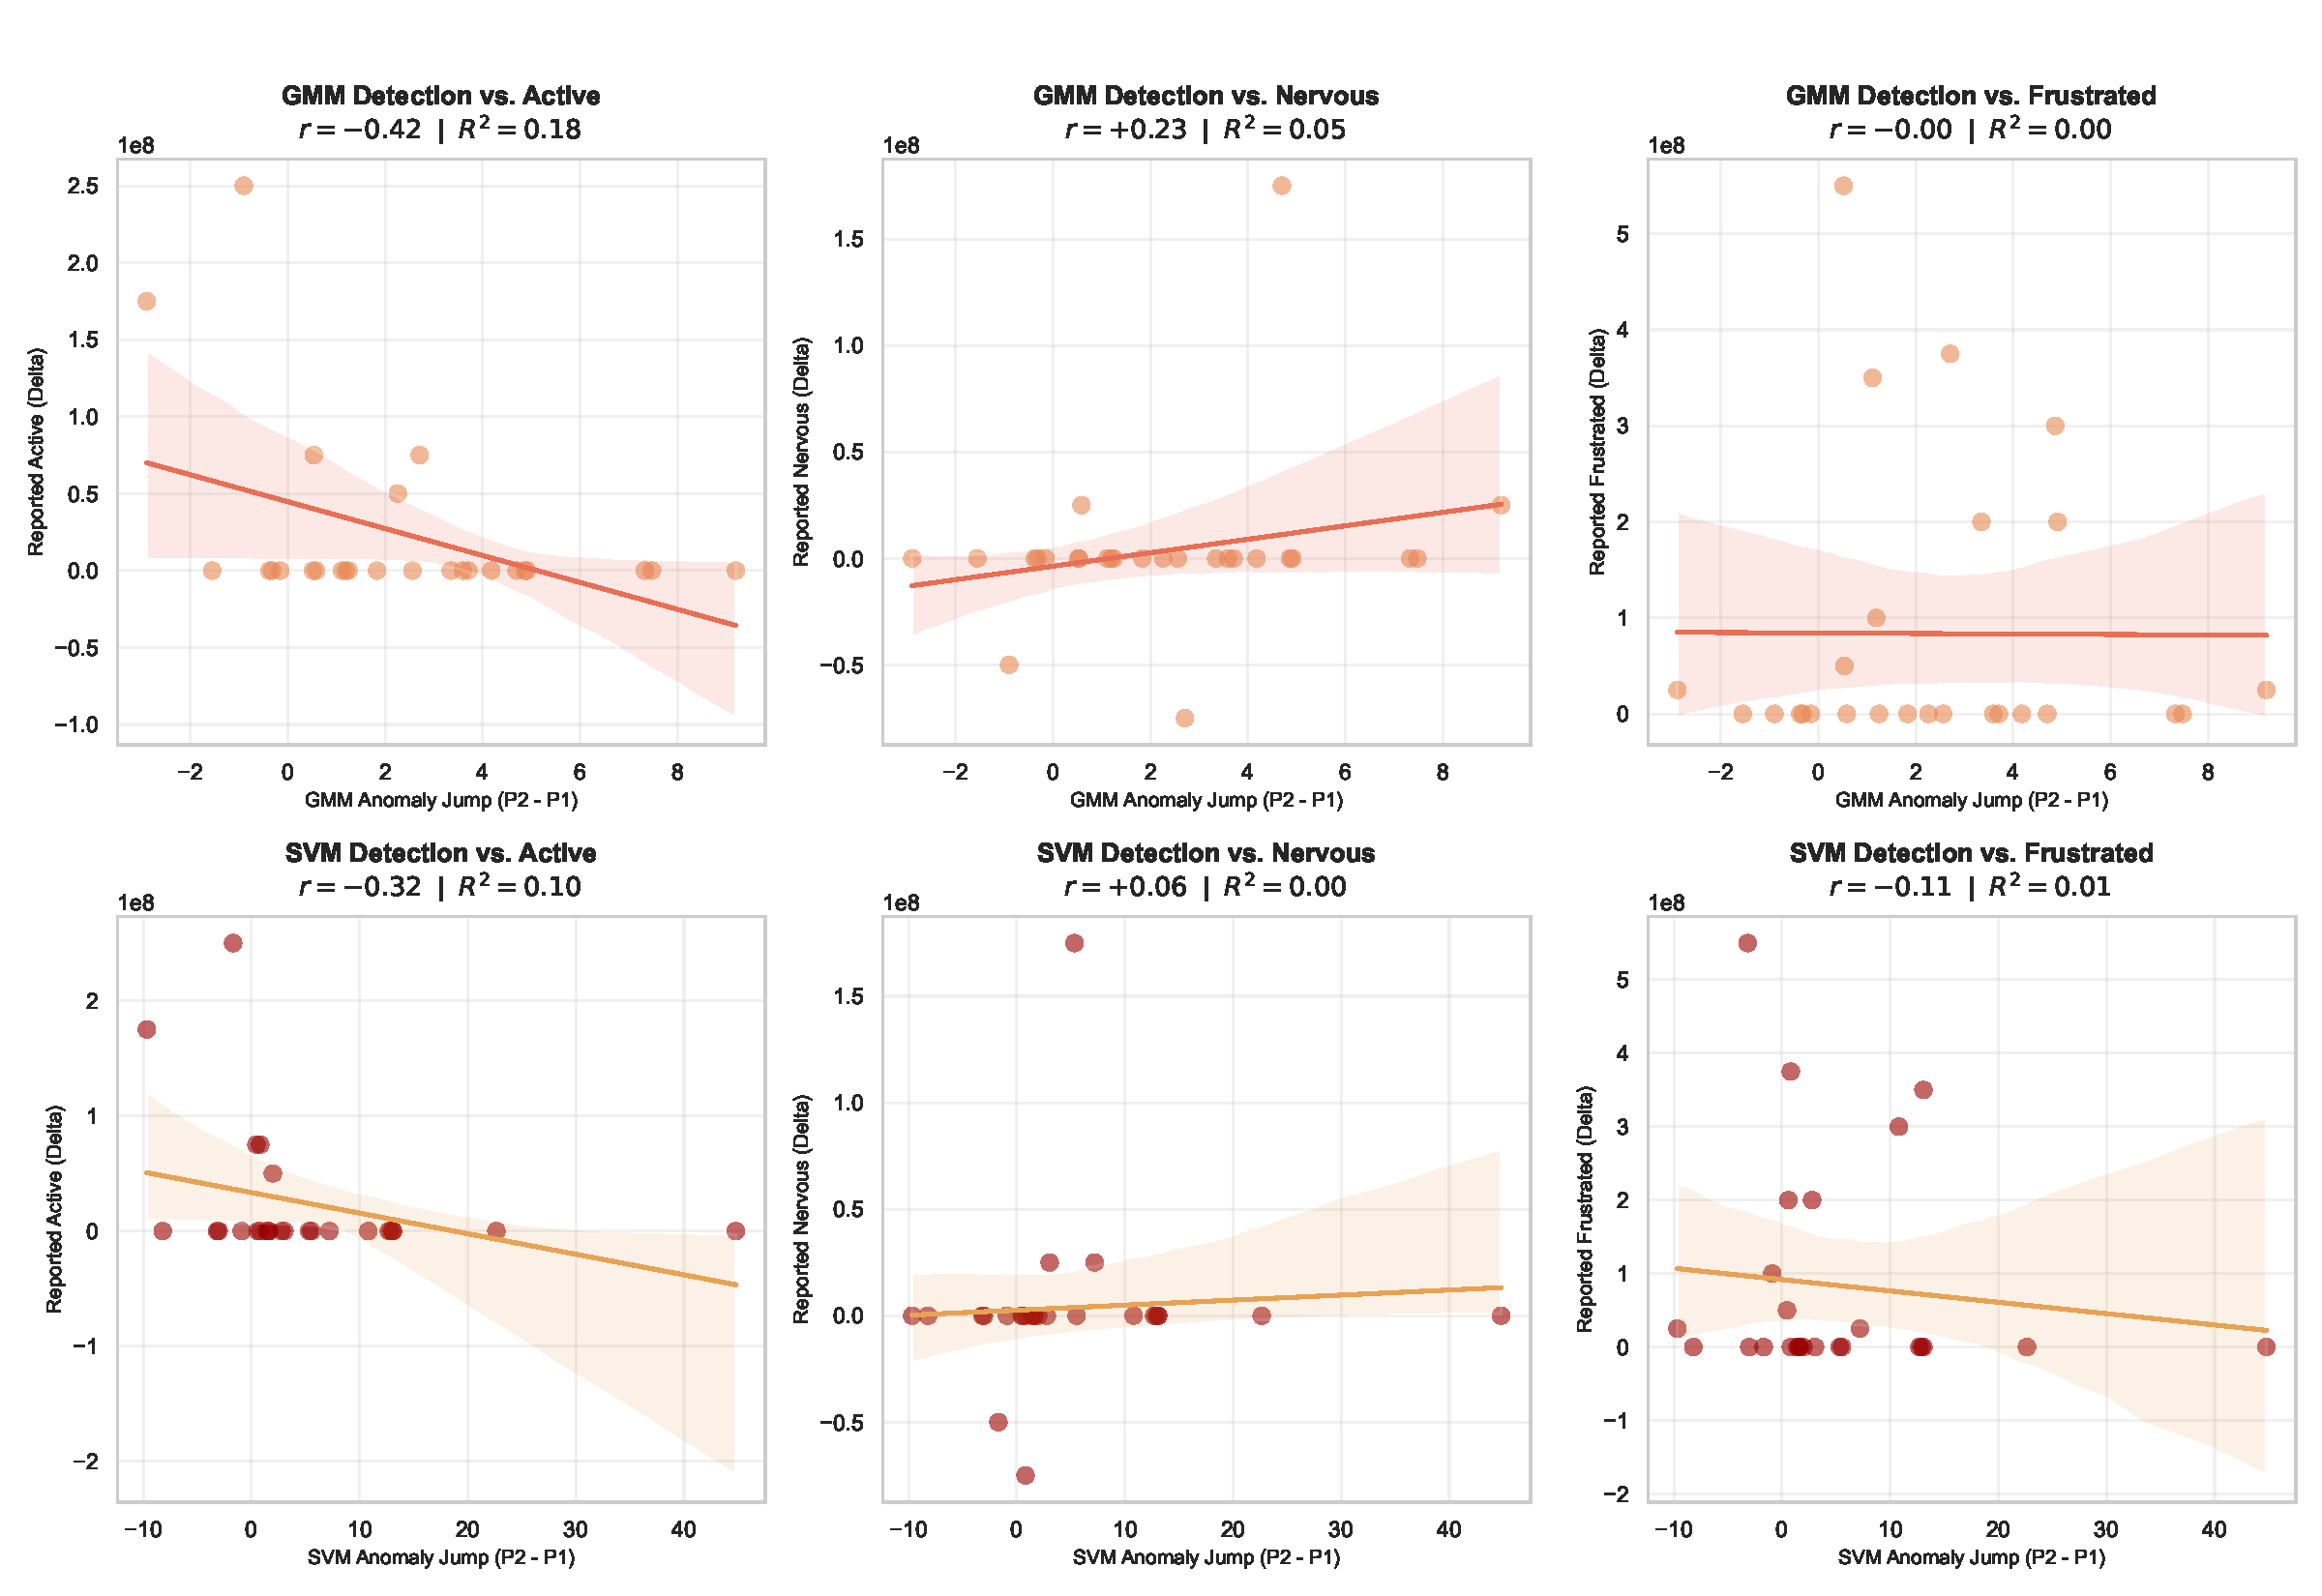
\includegraphics[width=0.99\linewidth]{figures/responses_correlation.pdf}
    \caption{Caption}
    \label{fig:responses_correction}
\end{adjustwidth}
\end{figure}


\section*{AI-aid use declaration}
\textcolor{red}{need to be written}



\section{Must be in report:}
 Written Report – Organization \& Structure:
*Layout is organized, effective, professional, and follows the provided template
* Clarity of content (clear research questions and transparent methodology)
\\
– Written Report – Technical Solution:
* Design and justification of the ML-pipeline (Data Pre-processing → Representation →
Evaluation)
\\
* Robustness of data handling (Clear justification for how missing values, scaling, and
specific data types were handled)
\\
* Validity of model validation (Correct methodology for estimating generalization eror/EPE, appropriate data splits)
\\
* Critical assessment of data quality, signal strength, and model limitations (e.g., properly
diagnosing a ’null result’ due to noisy data)
\\
* Originality, rigor, and complexity of method (Note: Rigorous evaluation of a simple
method is valued as highly as a complex method)
\\
* Quality of results (How well does the method solve the problem, or how well are the
limitations/weak signals explained?)
\\
* The method supports the main points (the aim)
\\
* Reproducibility and code quality (Repository is linked, code is readable and organized


\newpage
\section{what we need to do}
\begin{itemize}
    \item SVM
    \begin{itemize}
        \item A (bar) plot from the SVM 
        \item Some numbers about performace SVM
        \item a table of the gammas and mus we use (gridsearch)
    \end{itemize}
    \item what happens to the missing values 
    \item read through the evaluation pdf so we know if we are lacking
    \item write about GMM
    \begin{itemize}
        \item rewrite the introduction to fit the GMM and SVM
        \item add small paragraph about PCA in preprocessing
        \item add a plot of performance to compare with SVM
    \end{itemize}
    \item poster is still missing model, results 
\end{itemize}

\newpage
\addcontentsline{toc}{section}{Discussion}
%\input{sources/3_Discussion}

\newpage
\addcontentsline{toc}{section}{References}
%\bibliography{document.bib} 
%\bibliographystyle{ieeetr}


\printbibliography


\newpage
%\section{Appendix A} \label{ch6}

\label{endOfDoc}
\end{document}